\documentclass[11pt, titlepage]{article}

% Language setting
\usepackage[english]{babel}

% Page format
\usepackage[a4paper]{geometry}
\linespread{1.5} 

% Header
\usepackage{fancyhdr}
\addtolength{\headheight}{1.5cm} % make more space for the header
\pagestyle{fancyplain} % use fancy for all pages except chapter start
\fancyhf{} % clear header text chapter
\rhead{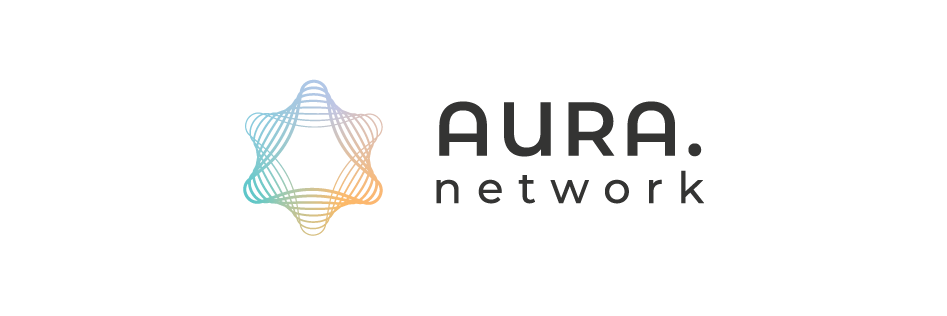
\includegraphics[height=1.3cm,trim={0cm 1.5cm 8cm 1.5cm} ]{img/logo.png}} % right logo
\rfoot{\thepage}
\renewcommand{\headrulewidth}{0pt} % remove rule below header

% Useful packages
\usepackage{amsmath}
\usepackage{graphicx}
\usepackage[colorlinks=true, allcolors=blue]{hyperref}
\usepackage[table,xcdraw]{xcolor}

% packages for vertical timeline
\usepackage[T1]{fontenc}
\usepackage[utf8]{inputenc}
\usepackage{charter}
\usepackage{environ}
\usepackage{tikz}
\usetikzlibrary{calc,matrix}
%% Code by Claudio:
%% https://tex.stackexchange.com/a/197447/221452
%% Uses code by Andrew:
%% http://tex.stackexchange.com/a/28452/13304
\makeatletter
    \let\matamp=&
    \catcode`\&=13
    \def&{%
        \iftikz@is@matrix%
            \pgfmatrixnextcell%
        \else%
            \matamp%
        \fi%
    }
\makeatother

\newcounter{lines}
\def\endlr{\stepcounter{lines}\\}

\newcounter{vtml}
\setcounter{vtml}{0}

\newif\ifvtimelinetitle
\newif\ifvtimebottomline

\tikzset{
    description/.style={column 2/.append style={#1}},
    timeline color/.store in=\vtmlcolor,
    timeline color=red!80!black,
    timeline color st/.style={fill=\vtmlcolor,draw=\vtmlcolor},
    use timeline header/.is if=vtimelinetitle,
    use timeline header=false,
    add bottom line/.is if=vtimebottomline,
    add bottom line=false,
    timeline title/.store in=\vtimelinetitle,
    timeline title={},
    line offset/.store in=\lineoffset,
    line offset=4pt,
}

\NewEnviron{vtimeline}[1][]{%
    \setcounter{lines}{1}%
    \stepcounter{vtml}%
    \begin{tikzpicture}[column 1/.style={anchor=east},
        column 2/.style={anchor=west},
        text depth=0pt,text height=1ex,
        row sep=1ex,
        column sep=1em,
        #1
    ]
        \matrix(vtimeline\thevtml)[matrix of nodes]{\BODY};
        \pgfmathtruncatemacro\endmtx{\thelines-1}

        \path[timeline color st]
            ($(vtimeline\thevtml-1-1.north east)!0.5!(vtimeline\thevtml-1-2.north west)$)--
            ($(vtimeline\thevtml-\endmtx-1.south east)!0.5!(vtimeline\thevtml-\endmtx-2.south west)$);

        \foreach \x in {1,...,\endmtx}{
            \node[circle,timeline color st, inner sep=0.15pt, draw=white, thick]
            (vtimeline\thevtml-c-\x) at
            ($(vtimeline\thevtml-\x-1.east)!0.5!(vtimeline\thevtml-\x-2.west)$){};
                \draw[timeline color st](vtimeline\thevtml-c-\x.west)--++(-3pt,0);
        }

        \ifvtimelinetitle%
            \draw[timeline color st]([yshift=\lineoffset]vtimeline\thevtml.north west)--
                ([yshift=\lineoffset]vtimeline\thevtml.north east);

            \node[anchor=west,yshift=16pt,font=\large]
                at (vtimeline\thevtml-1-1.north west)
                {\textsc{Timeline \thevtml}: \textit{\vtimelinetitle}};
        \else%
            \relax%
        \fi%

        \ifvtimebottomline%
            \draw[timeline color st]([yshift=-\lineoffset]vtimeline\thevtml.south west)--
            ([yshift=-\lineoffset]vtimeline\thevtml.south east);
        \else%
            \relax%
        \fi%
    \end{tikzpicture}
}

% Fix too long hyperlinks in bibliography
\usepackage{url}
\def\UrlBreaks{\do\/\do-}

\begin{document}
\title{Aura Network:\\
an NFT-centric blockchain platform}
\author{
admin@aura.network\\
nam.phan@aura.network}
\date{\today}
\maketitle

\tableofcontents
\newpage
% \begin{abstract}
% Your abstract.
% \end{abstract}

\textit{
This paper gives an overview of \emph{Aura Network}, a layer-1 NFT-centric blockchain platform. Aura focuses on chain optimization for NFT use cases, helping artists and other content providers to create a new, user-friendly experience with their digital assets. Aura is built using Cosmos SDK, the most popular framework for building blockchains, that powers BNB Smart Chain, Terra, Cosmos Hub, and many other chains.
}

\section{Context}

Since the birth of Bitcoin in 2009, the crypto market has grown to thousands of billions of US dollars in size. While most on-chain activities come from decentralized finance (DeFi), we have seen unprecedented growth in the popularity of non-fungible tokens (NFT) since the last year. An NFT is a distinguishable token that can be owned and transacted by individuals. 
Given an asset, either digitized or physical, we can issue an NFT that embeds the asset metadata including name, description, and images to represent the ownership of the NFT creator to such asset. As this ownership relation can be freely traded in the market and the unique property of the token, NFT investment is becoming widely popular. By the last quarter of 2021, the NFT sales worldwide have surged to \$ 10.5 Billion \cite{nftsale}. 

NFT is growing beyond simple collectibles towards a much more diverse use of NFTs in finance, gaming, real estate, metaverse, etc. Every asset, digital or physical, can have its unique representation in the decentralized blockchain ecosystem and can be transacted without restriction. A lot of new applications and platforms rise to tackle new use cases or target different communities. These solutions have to overcome a lot of challenges before becoming actually mainstream, especially in terms of usability and interoperability. 

\emph{Usability} is a key factor in almost all software products that end-users interact with. While NFT is just a token standard, the actual NFT object is owned and transacted by end-users through various decentralized applications (DApps). Most of the current NFT schemes are based on Ethereum, thus they inherit drawbacks such as low throughput, expensive transaction fees, and environmental impact, from the Ethereum network as well. While the Ethereum community is working towards a more scalable and sustainable ecosystem with \emph{Eth2}, it is still a long way until all the upgrades are in place. Alternatively, other blockchains with much better usability emerge such as Flow or BNB Smart Chain (BSC). While non of the alternative choices is as popular as Ethereum, these blockchain platforms offer a much better user experience and are more suitable for different use cases. 

There is little \emph{interoperability} among different NFT ecosystems. There is currently no way to directly transmit an NFT from Ethereum to BSC yet. While cross-chain communications are blooming, it is still some time before we can see all of these advancements work with NFT. While the major NFT schemes are concentrated in Ethereum, this problem prevents the wide adoption of the technology to other blockchain platforms.

What is the most popular blockchain platform for NFT? Despite all drawbacks in the usability of Ethereum, NFT transaction value on the platform still dominates the market by more than 85\% (March 2022)~\footnote{https://cryptoslam.io/}. Following the chart are Ethereum competitors such as Solana, Avalanche, etc. There is little difference between creating NFT on one platform and another. Hence it is extremely difficult for these platforms to compete with Ethereum as users are already much familiar with all the tools, wallets, and high liquidity marketplaces like OpenSea. Top blockchain platforms like Solana, BNB smart chain, Avalanche, etc. are having their own NFT marketplaces and games, mostly by investing a lot of capital in startups, game studios, or leveraging their existing crypto community.

When a business chooses a blockchain to create NFT, there are several things to consider such as transaction cost, robustness, security, speed, community, usability, interoperability, etc. It is difficult to have one that gets all of these characteristics. Some NFT projects that thrive to reach the next level of innovation choose another approach, that is to make their own blockchain network e.g. Ronin and Flow so that they can optimize and tailor it to have their desired quality. We believe that this bottom-up approach is the correct way of solving the usability and interoperability problems described above. There should be more layer-1 blockchains that can be optimized for specific purposes, governance and secured by communities that share the same trait or interest. Thus, applications on top of these blockchains can have more customization for their target customers. Eventually, these chains can be connected through various cross-chain communication protocols to create a network effect to bring more utility for tokens.

\section{Introducing Aura Network}

We introduce \emph{Aura Network}, an NFT-centric, layer-1 blockchain that focuses on expanding the use of NFT across various industries. Our vision is to create a one-stop destination for minting, evaluating, querying, and transacting NFT, to become a pioneer NFT infrastructure for the future. Aura Network focuses on building a \emph{sovereign blockchain} that is optimized for NFT use cases. This section provides a high-level view of the vision of Aura Network.

\subsection{Sovereign blockchain}
Aura Network is a \emph{sovereign blockchain}. That means having its own decentralized infrastructure that can be governed independently by Aura Community rather than depending on other layer-1 chains. Ecosystems like Ethereum or Solana are trying to have everything built on top of it, this makes these networks eventually be congested with too many unrelated transactions that can only be solved by sacrificing either security or decentralization. Even then, it takes a long time to update these networks as every change might cause a significant impact on existing applications. By building a sovereign, NFT-centric blockchain, Aura will have more freedom to optimize the platform to give better performance, security and utility for NFT applications. 

\subsection{Optimizing and scaling for IP owners}
Aura focuses on helping \emph{brands}, \emph{influencers}, \emph{IP owners}, and \emph{game creators} by providing a way to tokenize their digital assets to create a unique experience using NFT. Aura's thesis on building the next level NFT eco-system evolves around this customer segment is as follows:

\begin{itemize}
    \item \textbf{Bottom-up optimization}: By working directly with content providers or owners, Aura gradually optimizes the platform both in terms of technical capacity and utilities for accelerating the building process of NFT based decentralized applications. 
    \item \textbf{Geological scaling}: Aura shares the view of Ethan Buchman - \emph{co-founder of Cosmos} on blockchain scalability via geo-local systems. It is to bridge the gap between the platform and the customer it serves by providing support for local communities. Eventually, successful applications building on top of Aura from one local community can be easily replicated and customized to fit other communities that share the same attributes such as culture, language, countries, etc.
    
    \item \textbf{Maximize interoperability}: Pushing bottom-up development is not scalable in the long term. Eventually, this approach will meet top-down systems like Ethereum or Solana at some point. By adopting global standards, integrating with bridges and inter-blockchain communication protocol, Aura can help local brands and content providers to scale their applications and products to the global market.
\end{itemize}

In developing this thesis, Aura is one of the pioneer platforms that help local businesses, IP owners and game studios to tokenize their portfolios and scale to a global level. This will help bring more end-users from the mainstream traditional market into the NFT/metaverse ecosystem. This is the key step in improving the awareness about and utility of NFT as it then can be used widely even in traditional finance.  

\subsection{A universal framework for NFT}
The original Ethereum token standards ERC-721 and ERC-1155 laid a foundation for NFT standard interfaces. How these tokens are created and used in DApps depends on the creativity of developers. It is also the source of complexity in developing DApps. There are well-known middleware solutions to tackle this complexity such as \emph{Infura} or \emph{Metaplex} but mostly they are tools and managed services helping application developers to outsource the complexity of key management or blockchain client integration. Aura Network takes it to the next level by not only developing middleware services and open-source smart contract templates but also supporting integration with local services such as payment gateways, e-commerce platforms, social networks, etc. With such built-in support tools, Aura Network helps to accelerate not only creating new DApps, but also creating a whole new NFT business easily. 

\subsection{Maximizing interoperability}

With the success of Bitcoin, Ethereum, Cardano, and others, a lot of crypto project was born, creating many isolated blockchain networks. With multiple blockchains coexisting, cross-chain communication solutions emerge. Atomic swap, cross-chain messages, inter-blockchain communication protocols are all examples of the capability to link different blockchains together to create a more cohesive ecosystem that benefits everyone. While most of the existing technique applies to fungible tokens, there are a lot of use cases for inoperable NFT that can be transferred from one chain to another for example digital assets, game items, deeds, identity, etc.

Interoperability is a key part of the thesis of building Aura Network. Inter-connectivity and bridging are major forces driving the success of DeFi and we expect it will be the same for NFT.

\section{Architecture}
In this section, we will present the high-level software architecture of the Aura Network ecosystem. 

\subsection{Blockchain Platform}
The Aura Network Blockchain platform is a \emph{Layer-1 blockchain} built using \emph{Cosmos SDK} \cite{kwon2019cosmos}. The Cosmos SDK is an open-source framework for building proof-of-stake blockchains. It allows developers to create a blockchain platform from scratch with interoperability with other blockchain platforms. 

\begin{figure}[ht]
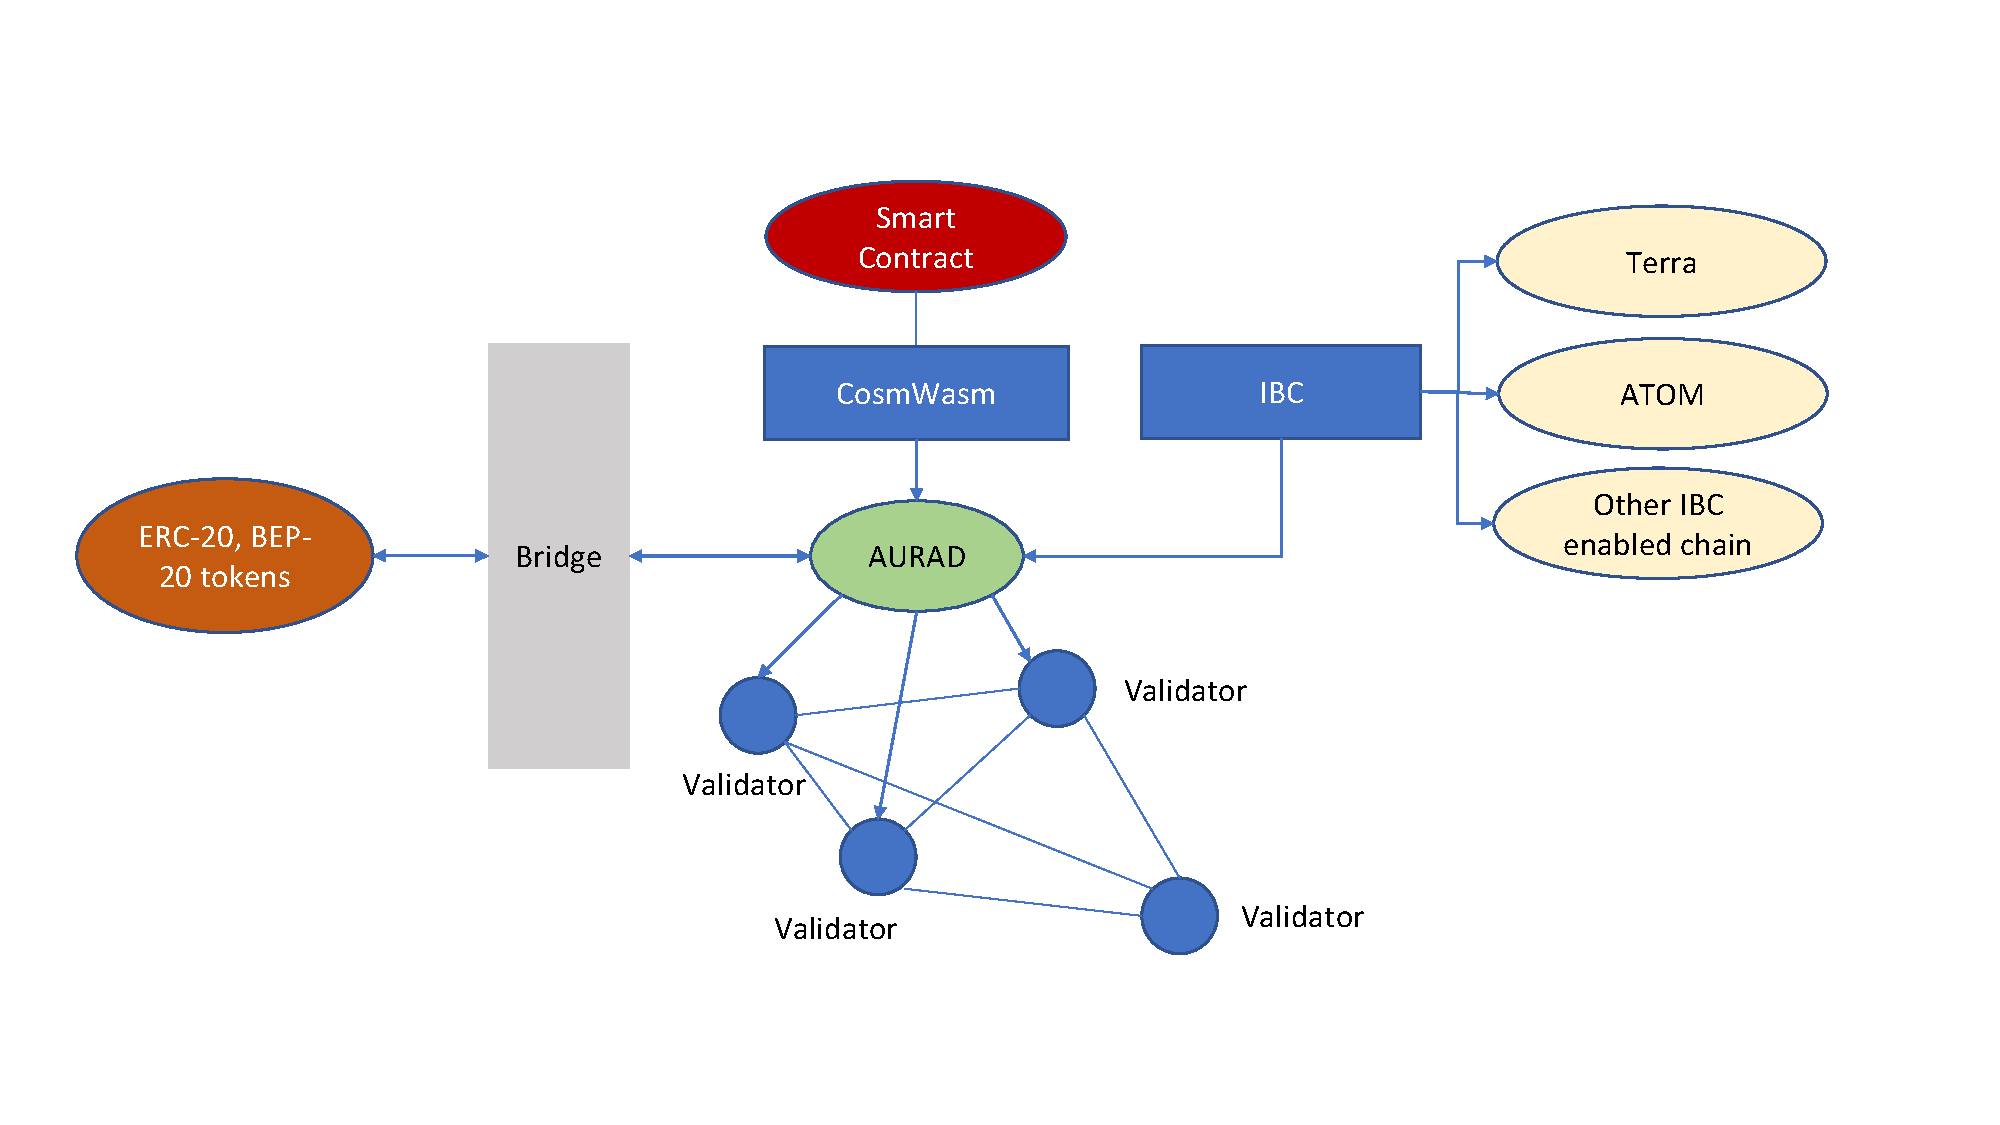
\includegraphics[width=\textwidth, trim={0 2cm 2cm 0}, clip]{img/architecture.pdf}
\centering
\caption{The Aura Network blockchain architecture}
\label{fig:architecture}
\end{figure}

Figure \ref{fig:architecture} shows the high-level architecture of the Aura blockchain platform. There are several main components that we want to highlight in this architecture:

\subsubsection*{Validator}
\emph{Validators} are blockchain nodes that participate in the consensus process to confirm transactions and produce blocks.
The consensus engine is \emph{Tendermint}~\cite{buchman2016tendermint}, a Byzantine Fault Tolerance state machine replication engine while the Proof-of-Stake (PoS) logic layer is provided by the Cosmos SDK. 

\subsubsection*{aurad}
\emph{aurad}, the short form of ``Aura Daemon" refers to the compiled platform binary that runs on all Validator nodes. aurad contains standard Cosmos modules like \emph{Auth}, \emph{Bank}, \emph{Mint}, \emph{Slash}, \emph{Stake}, etc. that are required to run the blockchain platform. There are a few simple modifications such as adding parameters and specific business logic that may be required by the Aura tokenomics. But overall, there won't be much change from the provided modules from Cosmos.

\subsubsection*{CosmWasm}
CosmWasm stands for ``Cosmos WebAssembly", it's a Cosmos module that enables WebAssembly virtual machines in the cosmos SDK. As the smart contract written for CosmWasm is compatible with all other Cosmos-based blockchains, we choose CosmWasm as the middleware for building smart contracts and DApps for the Aura ecosystem. Currently, it only supports contracts written in \emph{Rust}, but many high-level programming languages can be added in the future.

\subsubsection*{IBC}
Inter-Blockchain Communication Protocol (IBC) is the signature Cosmos module that supports transferring tokens directly from one chain to another. Aura Network enables IBC by default so that moving Aura Coin to Terra, Atom, Osmosis or other IBC-enabled blockchains can be performed easily.

\subsubsection*{Bridge}
Bridge is also an important part of aurad. As Aura Network focuses on bridging assets to other blockchains even outside of the Cosmos SDK, bridge solutions that support ERC-20, BEP-20 tokens will be employed. We are in contact with some decentralized exchanges and bridge teams e.g. Impossible Finance to develop this component. 

\subsection{Aura Network ecosystem}
Figure~\ref{fig:auraeco} shows the building blocks of the Aura Network. At the moment, we divide the ecosystem into 4 main categories

\begin{figure}[ht]
\label{fig:auraeco}
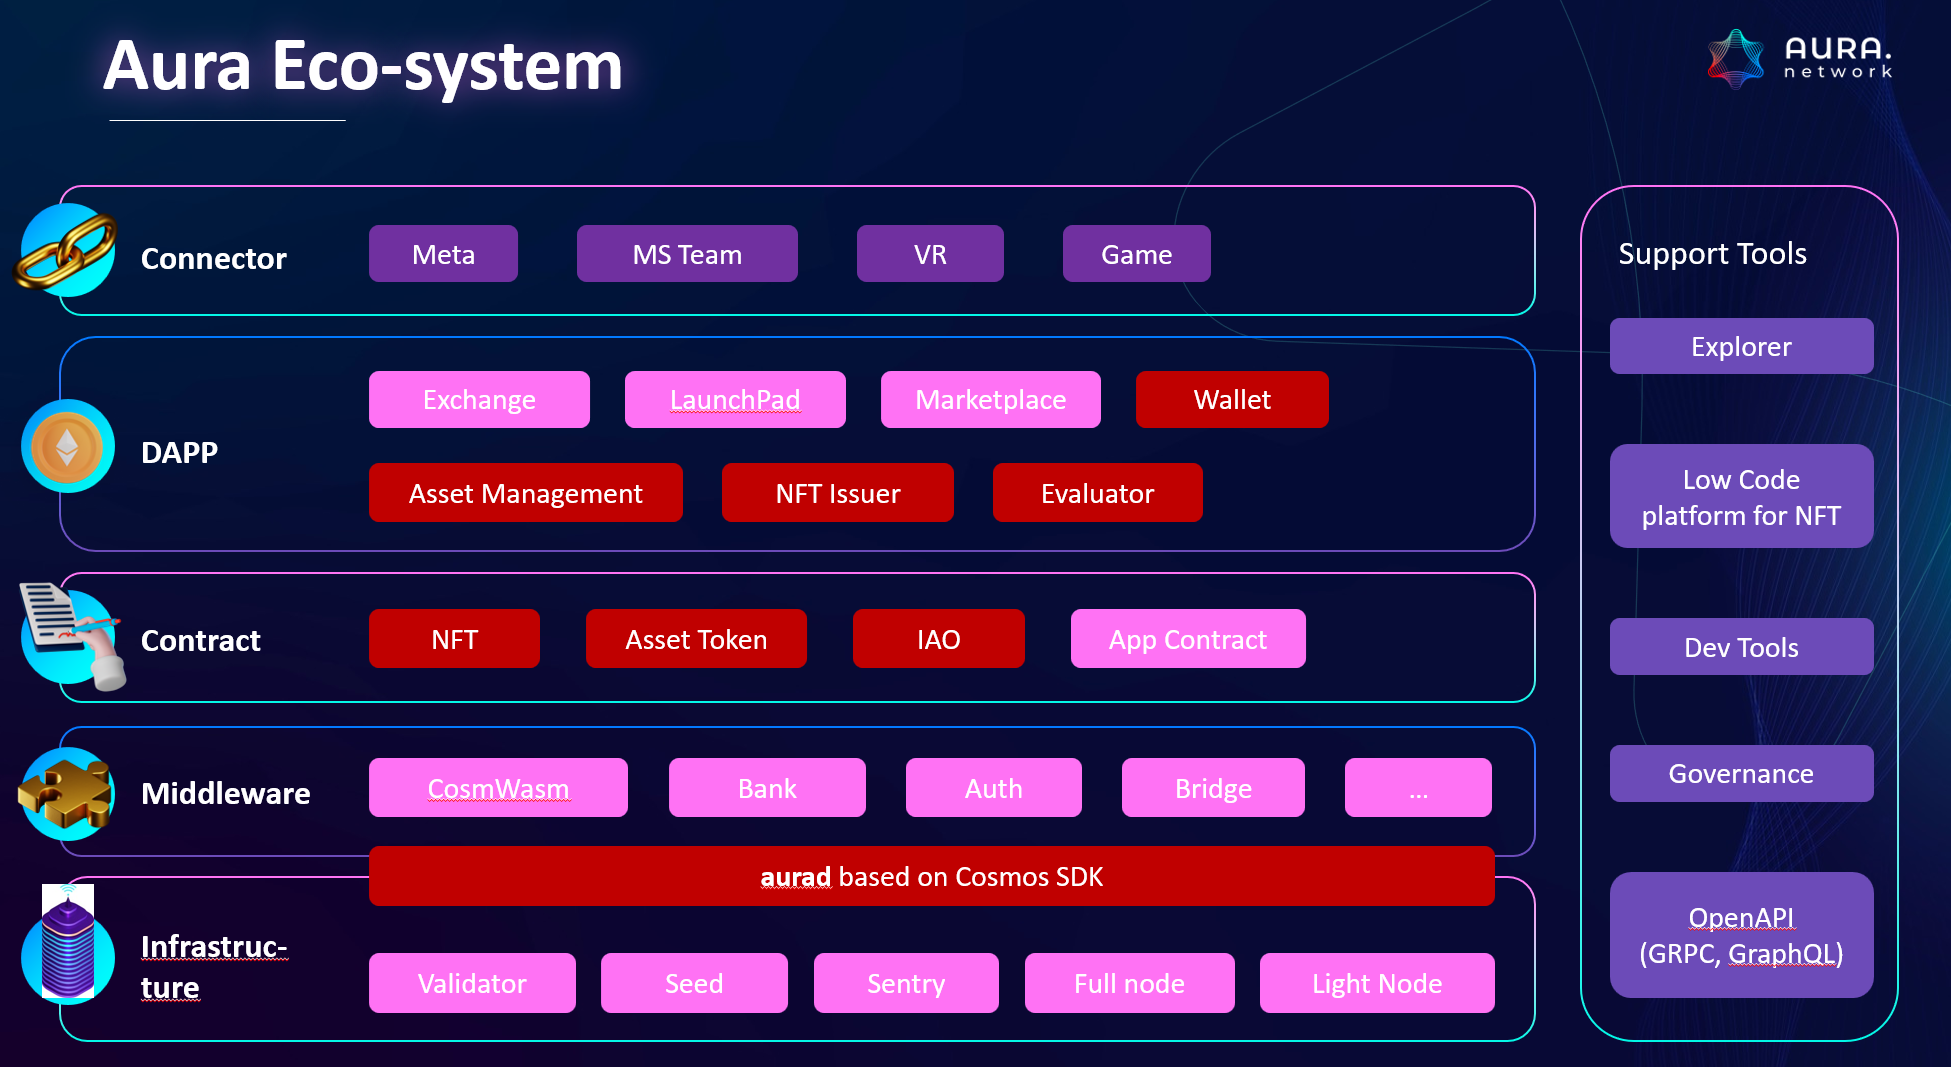
\includegraphics[width=18cm, trim={5cm 3cm 0cm 2cm}]{img/auraeco.png}
\centering
\caption{The Aura eco-system}
\end{figure}

\subsubsection*{Infrastructure}
The Infrastructure layer mostly refers to the blockchain platform that is mentioned above. Other than validators, Cosmos and Tendermint's best practices in running production software also include Seed, Sentry, Full and Light nodes. Details on the setup of these nodes are described in the Cosmos SDK documentation. We will also provide scripts and instructions on how to set up different types of nodes later on through Aura development documents. The \emph{Aura Daemon} client, or \emph{aurad} refers to the application running Aura Network.
Most of the provided Cosmos modules are included in aurad. Modifications to these modules are documented in the development docs.

\subsubsection*{Currency}
There are 2 native currencies of the Aura ecosystem: Aura Coin and Aura Token on BNB Smart Chain. Details about these currencies are specified on the tokenomic section. Aura also supports creating CW20 tokens, similar to other blockchains that use CosmWasm module.

\subsubsection*{Decentralized App}
Decentralized Applications (DApps) are the main focus of the Aura Network. These applications offer rich user experience in working with crypto currencies and NFT in general.

\begin{itemize}
    \item \textbf{AuraScan}: the blockchain explorer with extra features for governing, staking, NFT, notifications, etc. that are tailored towards Aura holders. 
    \item \textbf{NFT Hub}: one-stop destination for Aura community to interact with NFT and metaverse.
    \item \textbf{Aura DEX}: decentralized exchange for CW-20 tokens building on Aura.
    \item \textbf{Playground}: web-based smart contract IDE for developers, inspired by Ethereum Remix IDE.
    \item \textbf{Bridge}: aura bridge for swapping assets between BSC and Aurachain.
    \item \textbf{Marketplace}: NFT marketplace
    \item \textbf{Launchpad}: Aura provides intensive supports both in terms of technology and funding, business promotion to NFT projects building on Aura chain
    \item \textbf{Aura Safe}: Gnosis-safe inspired multisignature wallet.
\end{itemize}

\subsubsection*{Open API}
The Open API layer contains integration APIs, SDKs that are used to bring NFT assets to Metaverse networks. By itself, Aura Network does not provide a metaverse experience but provides infrastructures for bringing NFT assets to the metaverse.

\section{Tokenomics}

This section describes information related to a native currency supported by the Aura Network.

\subsection{Token Usage}
We introduce 2 types of native tokens in the Aura Network: the Aura Token on BNB Smart Chain and Aura Coin.

\subsubsection{Aura Token on BSC}

Before launching Mainnet, Aura first introduces the BEP-20 Aura Token on BNB Smart Chain. This token acts as a placeholder for the later Aura Coin that will be introduced when Aura Mainnet launches. Like other BEP-20 tokens, Aura Token can be freely traded on the cryptocurrency market. Aura Token also helps provide liquidity on BEP-20 compatible decentralized exchange and bootstrap users from this community.

\subsubsection{Aura Coin}
Aura Coin is the native currency of the Aura Network blockchain platform. Besides the trading capability of Aura Token, Aura Coin has many other utilities:

\begin{itemize}
    \item \textbf{Staking}: Aura Coin holders can delegate their coins to trusted validators to earn passive commission income from the network.
    \item \textbf{Governing}: Aura Coin holders can participate in voting for software updates or other important decisions on how the Aura community should be developed.
    \item \textbf{Transaction fee}: Aura Coin is used to pay for transaction fee.
    \item \textbf{Exchange and Swap}: Aura Coin can be exchanged or swapped in the market.
\end{itemize}

\subsection{Token Distribution}

% Please add the following required packages to your document preamble:
% \usepackage{graphicx}
% \usepackage[table,xcdraw]{xcolor}
% If you use beamer only pass "xcolor=table" option, i.e. \documentclass[xcolor=table]{beamer}
\begin{table}[]
\centering
\resizebox{\textwidth}{!}{%
\begin{tabular}{|l|l|l|l|l|l|}
\hline
\rowcolor[HTML]{000000} 
{\color[HTML]{FFFFFF} \textbf{Token   Allocation}} & \multicolumn{1}{c|}{\cellcolor[HTML]{000000}{\color[HTML]{FFFFFF} \textbf{Allocation   (\%)}}} & \multicolumn{1}{c|}{\cellcolor[HTML]{000000}{\color[HTML]{FFFFFF} \textbf{\$AURA}}} & \multicolumn{1}{r|}{\cellcolor[HTML]{000000}{\color[HTML]{FFFFFF} \textbf{TGE}}} & \multicolumn{1}{r|}{\cellcolor[HTML]{000000}{\color[HTML]{FFFFFF} \textbf{Token TGE}}} & {\color[HTML]{FFFFFF} \textbf{Vesting Schedule (monthly)}} \\ \hline
\begin{tabular}[c]{@{}l@{}}Ecosystem   Growth \\ (ignore in circulating supply)\end{tabular} & 21.25\% & 212,500,000 & 30\% & 63,750,000 & linear   vesting over 2 years \\ \hline
Ecosystem Growth - listing DEX & 1.75\% & 17,500,000 & 100\% & 17,500,000 & no vesting \\ \hline
Strategic & 13.00\% & 130,000,000 & 0\% & 0 & linear   vesting over 2 years \\ \hline
Private   Sale round 1 & 2.16\% & 21,600,000 & 2\% & 432,000 & linear   vesting over 2 years \\ \hline
Private   Sale round 2 & 0.60\% & 5,957,500 & 5\% & 297,875 & linear   vesting over 2 years \\ \hline
Block   Rewards & 25.00\% & 250,000,000 & 0\% & 0 & rewards over 5 years \\ \hline
Team   and Advisors & 20.00\% & 200,000,000 & 0\% & 0 & 1 year cliff then linear vesting over 3 years \\ \hline
Public   Distribution & 1.25\% & 12,538,462 & 100\% & 12,538,462 & no vesting \\ \hline
\begin{tabular}[c]{@{}l@{}}Foundation   Reserves \\ (ignore in circulating supply)\end{tabular} & 14.99\% & 149,904,038 & 0\% & 0 & linear   vesting over 2 years \\ \hline
\textbf{Total} & \textbf{100.00\%} & \textbf{1,000,000,000} & \textbf{} & \textbf{94,518,337} & \textbf{} \\ \hline
\end{tabular}%
}
\caption{\label{tab:tokenomics}Aura Network tokenomics}
\end{table}

Table~\ref{tab:tokenomics} shows the token distribution metrics for Aura Network. The maximum amount of Aura that can be minted is exact \textbf{1 Billion} tokens. This value is specified in the Aura genesis block and cannot be changed in the future unless we do a hard fork. This is applied for both Aura Token on BSC and the Aura Coin as the token is simply just a placeholder. There are 6 categories that Aura coin will be allocated to:

\subsubsection{Ecosystem Growth}
23 percent of the total coin will be allocated to the ecosystem growth fund. This fund is used for ecosystem development such as project grants, bug bounties, attracting stakeholders to provide utility services, etc. Examples include, but are not limited, to the following: 

\begin{enumerate}
\item \textbf{Airdrop:} \\ 
Built on the Cosmos SDK system, we would like to reach the most active participants on the same system. As such, some AURA tokens will be dropped to ATOM and other tokens in the Cosmos system. The drop is either in a fixed quantity (in the spirit of Uniswap), or proportional to staked tokens. Tokens are claimable conditional on some criteria such as the length of staking, the minimum quantity of qualified tokens staked, participation in governance voting, or engaging with the community in any social media such as Telegram or Discord, etc. We will also consider airdropping some random Fan Tokens to AURA token holders to encourage people to hold AURA tokens on a long-term basis.
\item \textbf{Community pool:} \\
Developing and expanding network reach requires tokens as a source of capital, which can be financed from the Community pool. A stakeholder (can be a validator, advisor, or influential participant of the network) can write up a proposal and specify the requested quantity of tokens, the purpose of using tokens, the timeline of the plan, and any expected result.  
The proposal is then to be voted “Yes” or “No” on the majority rule basis. That is, if a proposal receives more than 50\% “Yes” votes, it will be implemented, and vice versa. The voter can be validators and/or token holders. Token holders can delegate their coin to their choice validator to increase the weight on the cast of that validator. The weight is proportional to the total amount of tokens available to all voters at the time of voting. The process is designed to be democratic, and proposals that are unambiguously beneficial to the network and stakeholders should pass most of the time.\\
There will be a time when a proposal is controversial in the sense that the benefit-cost is ambiguous to the voters. As such, we would like to collect feedback from the “No” voters on why they downvote the proposal. We propose that when choosing “No”, there is another question for why the voters choose no, and the answer is to be chosen in a multiple-choice format. This mechanism would help proposers to improve on their proposals for the following-up rounds.
 
\item \textbf{Bug bounty}: \\ 
Some tokens will be allocated to users who report bugs and propose fixes to the network.

\end{enumerate}

\subsubsection{Strategic Fund Raising}
20\% percent of the tokens go to private sales to strategic partners. They are invited to finance the project in an exchange for the token of a network, at a discount rate to compensate for the extra risk that they take in due to the projects being in the early stage. The strategic fund raising part is divided into Strategic Round, Private Sale Rounds. Leftover tokens from these rounds are merged to the foundation reserves pool.
 
\subsubsection{Public distribution}
We are working with several exchanges and launchpads to launch an Initial Exchange Offering (IEO) or an initial DEX offering (IDO). Aura is intended to be listed on both CEXs and DEXs to reach a wider range of investors. 

\subsubsection{Foundation Reserve}
The remaining of the total coin will be stored in the foundation treasury fund. It is supposed to be served as a “last-resort” in the case that the network requires funds to solve a particular problem that another source of funding (e.g Community Pooling) is not on the table. All decisions on how to spend the fund must go through a public governance proposal as outlined in the “Community Pool” subsection.
 
\subsubsection{Team}
20 percent of the total coin goes to the AURA team to incentivize the developer to expend their effort in building the network.
 
\subsubsection{Block Rewards}
25 percent of the total coins will be periodically minted as block rewards to distribute to validators and delegators. Incentives play a big role in deciding the token allocation. For example, allocating “insufficient” amount of tokens to validators may lead to the extreme case where validators cheat the network by accepting fraudulent blocks (e.g double-spending), or validators may not be interested in participating the network which threats the network security. Allocating too little tokens to advisors may result in advisors being “inactive”, discouraging them from engaging with the team to provide helpful advice. Overall, we strategically allocate our token in line with our long-term vision with regard to the development and future of the project, 

In the first \emph{5 years} of Mainnet, a total of 250 million Aura Coins will be distributed for validators in every block. Apart from the block rewards from the network, validators also receive transaction fees (\emph{gas}) from transaction creators. We assume that after 5 years of running Aura Network, the transaction fee from the network will be large enough to reward validators so there will be no need for block rewards to be minted anymore.

\subsubsection{Token generation event}
There are 2 \emph{Token Generation Events} (TGE) that are corresponding to the 2 types of native currency in the network, the token and the coin. For Aura Token on BSC, the token generation is quite standard as the Aura team will mint and transfer tokens manually based on the specification in Table~\ref{tab:tokenomics}.

By the time of Aura Mainnet's release and the listing of Aura Coin, the Aura Token contract on BSC will be frozen so that no more token can be minted. Aura Token holders then can claim their coins on the Aura Mainnet by sending their tokens on BSC to the migration contract. These tokens can be burnt later on. The state of the vesting schedule at the time will also be replicated on Aura Mainnet. 

\subsubsection{Account Vesting}
Vesting refers to the process of locking a certain amount of coins or tokens then gradually releasing them with time. Other than public distribution coins, the rest of the token allocation categories are locked and vested on different terms. The vesting process for Aura Token and Aura Coin starts at the IEO event. Tokens or Coins are linearly unlocked every month based on the vesting schedule. 

In Aura Mainnet, locked Tokens from Team and Strategic partners can still be delegated for staking and voting for governance. However, tokens in the ecosystem growth and foundation reserves are not available for delegation. 

\section{Roadmap}

\begin{vtimeline}[description={text width=12cm},
    row sep=4ex,
    use timeline header,
    timeline title={Aura Network Roadmap}]
    \textbf{2021} & -------- \textbf{Bootstrap \& Private Fundraising} -------- \endlr
    November & Establish project\endlr
    \textbf{2022} & -------- \textbf{Establishing Infrastructure} --------\endlr
    Q1 & Strategic Round\endlr
    Q2 & Aura Testnet, Wallet, Explorer, Multi-signature Wallet, Smart Contract support, NFT contract.\endlr
    Q3 & Aura Mainnet, Governance Tool, IBC enablement for native tokens\endlr
    Q4 & First NFT use case\endlr
    \textbf{2023} & -------- \textbf{Expanding the Network} --------\endlr
    TBD & IBC for NFTs, Metaverse integration, game support\endlr
\end{vtimeline}

\bigskip
\bigskip

We presents the roadmap of the Aura Network project in the timeline drawing above. From 2021 to 2023, the project goes through 3 main phases. The \emph{Bootstrap \& Private Fundraising} phase is in 2021 where the team perform mandatory steps to establish the project base such as registering legal entities, call for seed \& strategic funding from VCs, etc. The second phase in 2022 consists of mostly infrastructure building objectives such as issuing tokens, releasing Mainnet and some support tools. We also target to have our first NFT use case at the end of 2022. Finally, the third phase in 2023 will focus on developing bridges to other networks and metaverse connectors.


%\section{Conclusion}

\bibliographystyle{plain}
\bibliography{references}

\end{document}